\section{Auswertung}
\label{sec:Auswertung}

\raggedright

In dem folgenden Kapitel wird, aus den in Kapitel \ref{sec:Messwerte} aufgetragenen
Messwerten, der HeNe-Laser auf Stabilität, Polarisation, TEM-Moden und Wellenlänge untersucht.

\subsection{Stabilität}

Das für die Stabilitätsbedingung benötigte Produkt $g_1g_2$ ist in Abhängigkeit von $L$ in
Abbildung \ref{fig:vorbereitung} aufgetragen. Für die Auswertung ist dabei die Kurve für die zwei
konkaven Spiegel mit $r=\SI{1400}{\milli\meter}$, sowie die Konfiguration aus planaren und konkaven
Spiegel von Bedeutung.

\begin{figure}[H]
  \centering
  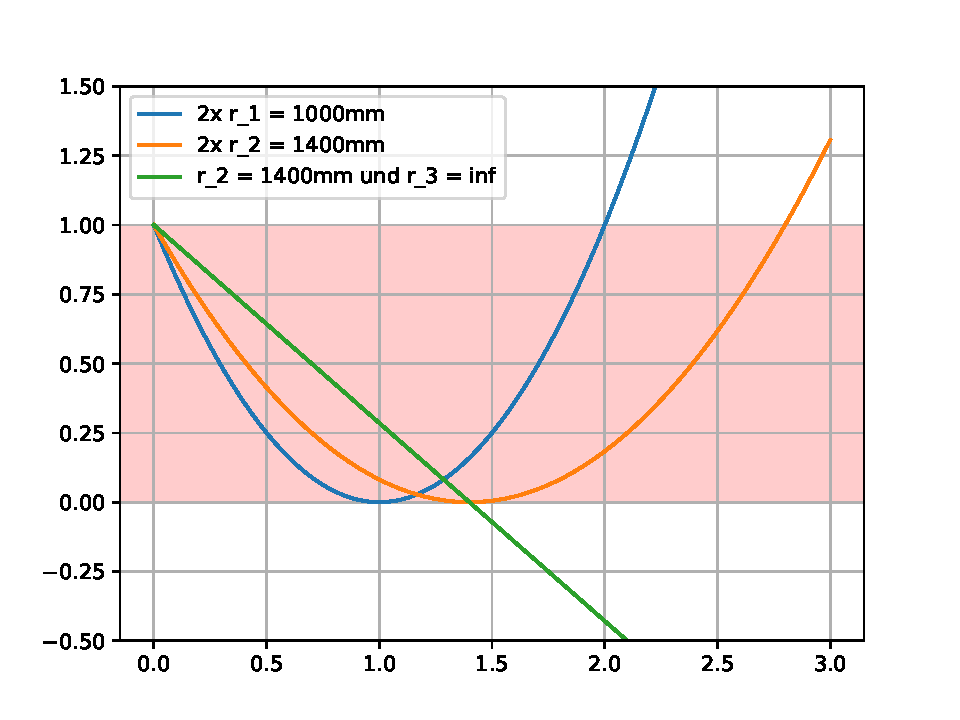
\includegraphics{vorbereitung.pdf}
  \caption{Stabilitätsbedingung für verschiedene Resonatorkonfigurationen.}
  \label{fig:vorbereitung}
\end{figure}

Die Messdaten für den Resonator mit dem planaren und konkaven Spiegel sind in Tabelle \ref{tab:planarkonkav}
aufgelistet.

An die Messdaten wird eine lineare Funktion mit den Parametern $a$ und $b$ gefittet:
\begin{align}
  I_{\symup{lin}}(L) = a\,\cdot\,L\,+\,b
\end{align}
Der Fit und die Messdaten sind in Abbildung \ref{fig:planarkonkav} abgebildet.

\begin{figure}[H]
  \centering
  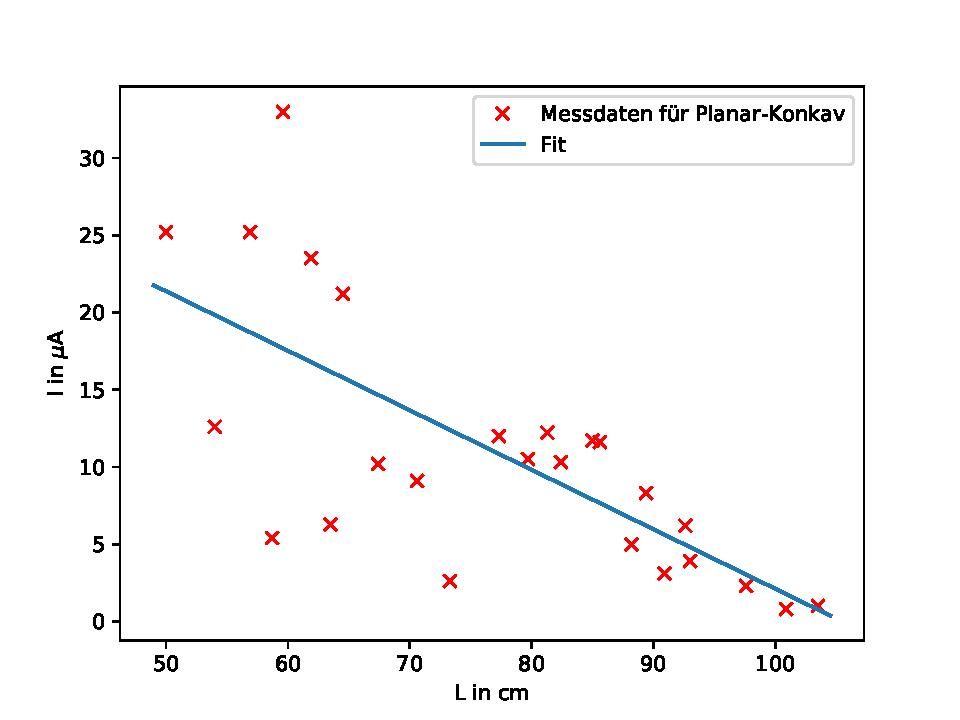
\includegraphics{stabilitaet_planarkonkav.pdf}
  \caption{Fit und Messdaten der planar-konkav Konfiguration.}
  \label{fig:planarkonkav}
\end{figure}

Aus dem Fit ergeben sich für die Parameter folgende Werte:
\begin{align}
  a &= \SI{-0.38(8)e-3}{\milli\ampere\per\centi\meter}\\
  b &= \SI{41(6)e-3}{\milli\ampere}\\
\end{align}

Die Messdaten für den Resonator mit zwei konkaven Spiegeln sind in Tabelle \ref{tab:konkavkonkav}
aufgelistet. Um einen möglichst quadratischen Verlauf zu erkennen, wurden für den Fit
nur die mit * markierten Werte verwendet.

Im Gegensatz zur planaren Konfiguration, wird in diesem Fall eine quadratische Funktion mit den
Parametern $a$, $b$ und $c$ an die Messwerte gefittet:

\begin{align}
  I_{\symup{quad}}(L) = a\,\cdot\,L^2\,+\,b\,\cdot\,L\,+\,c
\end{align}

In Abbildung \ref{fig:konkavkonkav} ist der Fit und die Messwerte gefittet.
Es ergeben sich folgende Werte für die Parameter:
\begin{align}
  a &= \SI{0.011(6)e-3}{\milli\ampere\per\centi\meter\squared}\\
  b &= \SI{-3(1)e-3}{\milli\ampere\per\centi\meter}\\
  c &= \SI{199(47)e-3}{\milli\ampere}\\
\end{align}
\begin{figure}[H]
  \centering
  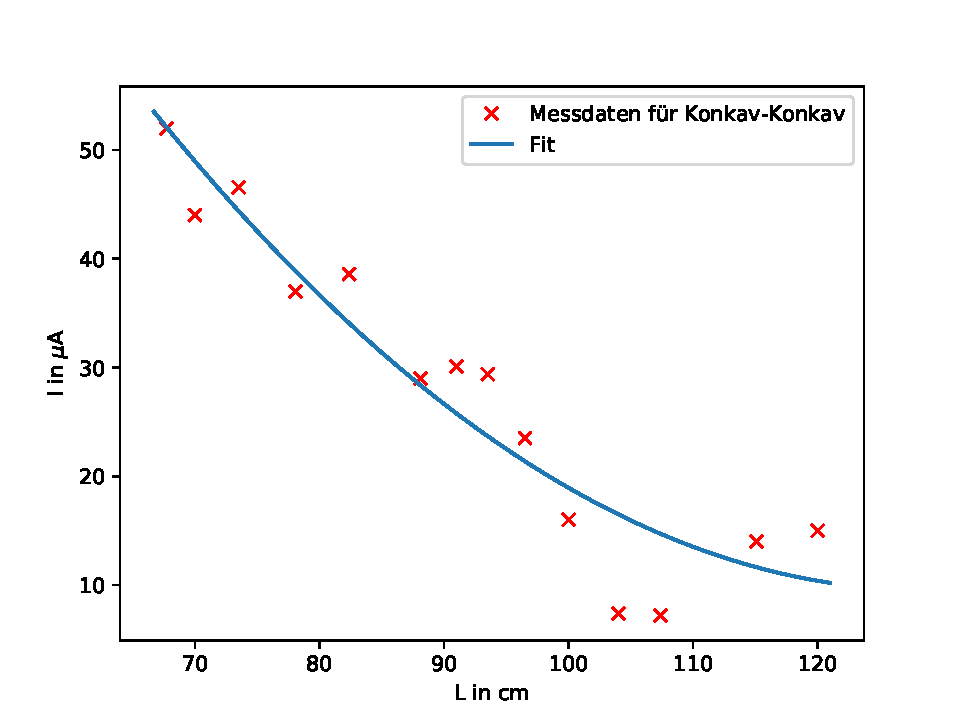
\includegraphics{stabilitaet_konkavkonkav.pdf}
  \caption{Fit und Messdaten der konkav-konkav Konfiguration.}
  \label{fig:konkavkonkav}
\end{figure}

\subsection{Polarisation}

Die Messdaten der Polarisationsmessung sind in Tabelle \ref{tab:polarisation} dargestellt.
Es wird eine Fitfunktion der Form
\begin{align}
  I_{\symup{pol}}(\varphi) = I_0\,\cdot\,\cos^2(\varphi-\varphi_0)
\end{align}
an die Messdaten gefittet, und so die Parameter $I_0$ und $\varphi_0$ bestimmt.

Der Fit und die Messdaten sind in Abbildung \ref{fig:polarisation} abgebildet. Für
die Parameter ergeben sich die Werte:
\begin{align}
  I_0 &= \SI{4.4(2)e-3}{\milli\ampere}\\
  \varphi_0 &= \SI{-0.40(4)}{\radian}\\
\end{align}

\begin{figure}[H]
  \centering
  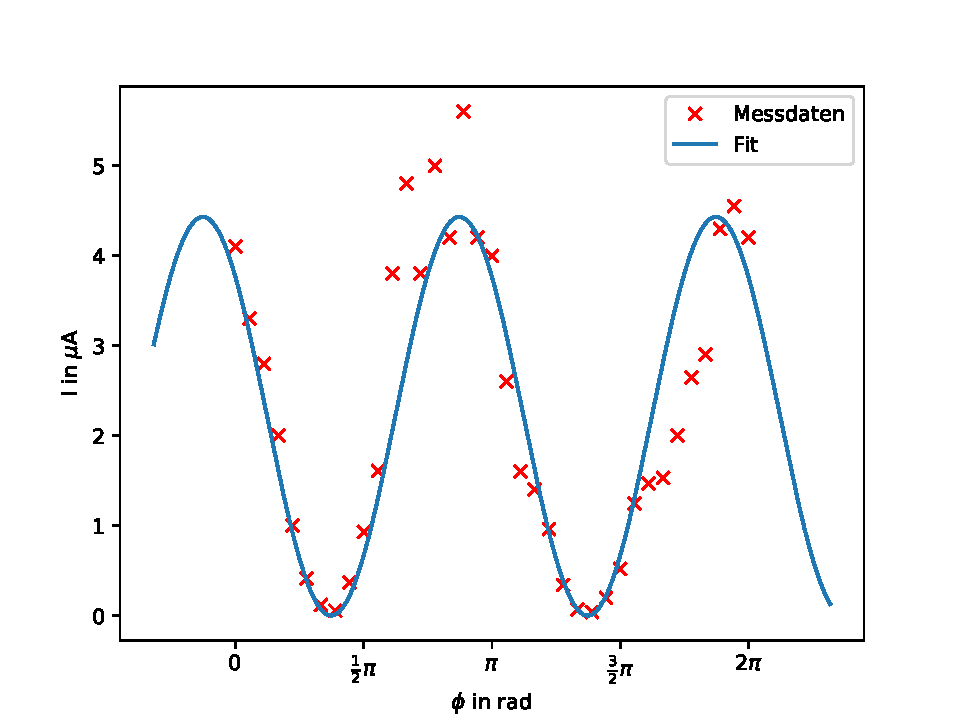
\includegraphics{polarisation.pdf}
  \caption{Fit und Messdaten der Polarisationsmessung.}
  \label{fig:polarisation}
\end{figure}

\subsection{TEM-Moden}

Die aufgenommenen Messdaten für die Grundmode sind in Tabelle \ref{tab:grundmode} aufgetragen.
Als Fitfunktion wird eine Gaußfunktion verwendet die die folgende Form hat:
\begin{align}
  I_{\symup{grund}}(L) = I_0\,\cdot\,\symup{exp}\left(-2\left(\frac{L-d_0}{\omega}\right)^2\right)
\end{align}

Dabei steht $d_0$ für die Verschiebung des Strahlmittelpunktes zum Nullpunkt der Skala.
Die Parameter $I_0$, $d_0$ und $\omega$ ergeben sich durch den Fit zu:
\begin{align}
  I_0 &= \SI{1.21(2)e-3}{\milli\ampere}\\
  d_0 &= \SI{-6.3(2)}{\milli\meter}\\
  \omega &= \SI{18.0(4)}{\milli\meter}\\
\end{align}

Der Fit und die Messwerte sind in Abbildung \ref{fig:grundmode} dargestellt.

\begin{figure}[H]
  \centering
  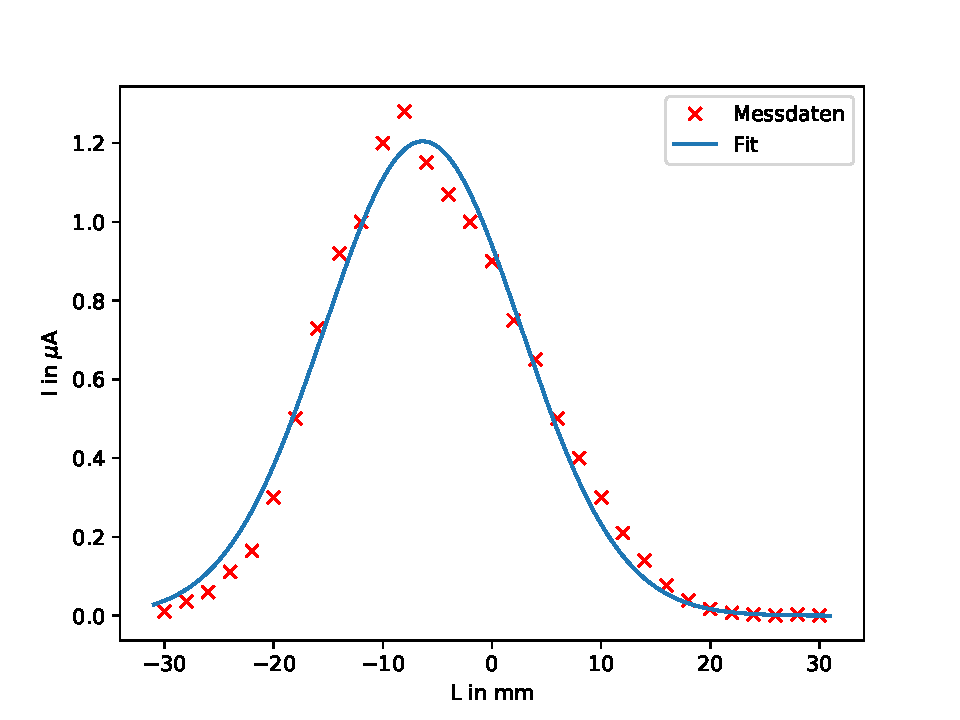
\includegraphics{grundmode.pdf}
  \caption{Fit und Messdaten der TEM-Grundmode.}
  \label{fig:grundmode}
\end{figure}

Die Messwerte für die erste Mode sind in Tabelle \ref{tab:erstemode} aufgetragen.
Als Fitfunktion wird eine asymmetrische doppelte Gaußkurve der Form
\begin{align}
  I_{\symup{erste}}(L) =
  I_{0,1}\,\symup{exp}\left(-2\left(\frac{L-d_{0,1}}{\omega_1}\right)^2\right)\,\,+\,\,I_{0,2}\,
  \symup{exp}\left(-2\left(\frac{
  L-d_{0,2}}{\omega_2}\right)^2\right)
\end{align}
verwendet.
Es ergeben sich folgende Parameter:
\begin{align}
  I_{0,1} &= \SI{97(2)}{\nano\ampere}\\
  d_{0,1} &= \SI{-14.9(1)}{\milli\meter}\\
  \omega_1 &= \SI{9.7(3)}{\milli\meter}\\
  I_{0,2} &= \SI{81(2)}{\nano\ampere}\\
  d_{0,2} &= \SI{7.9(2)}{\milli\meter}\\
  \omega_2 &= \SI{10.3(3)}{\milli\meter}\\
\end{align}

Der Fit ist in Abbildung \ref{fig:erstemode} dargestellt.

\begin{figure}[H]
  \centering
  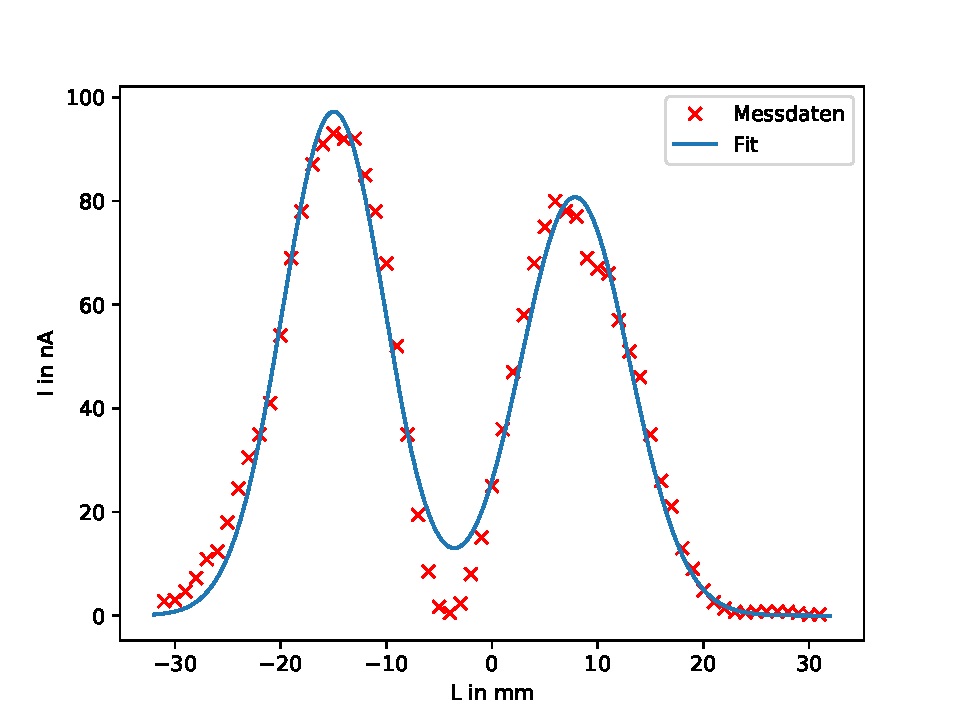
\includegraphics{erstemode.pdf}
  \caption{Fit und Messdaten der ersten TEM-Mode.}
  \label{fig:erstemode}
\end{figure}

\subsection{Wellenlänge}

Zur Bestimmung der Wellenlänge des HeNe-Lasers wird die Länge $L_1$ vom Gitter (mit Gitterkonstante a)
zum Maximum 0.ter Ordnung, sowie die Abstände $L_{2,1}$ und $L_{2,2}$ vom Maximum 0.ter Ordnung
zu den Maxima 1.ter Ordnung benötigt:
\begin{align}
  a &= \SI{1/100}{\milli\meter}\\
  L_1 &= \SI{67}{\centi\meter}\\
  L_{2,1} &= \SI{4.2}{\centi\meter}\\
  L_{2,2} &= \SI{4.25}{\centi\meter}\\
\end{align}
Aus den Längen $L_{2,1}$ und $L_{2,2}$ wird der Mittelwert $L_2$ gebildet, und somit über folgende
Formel die Wellenlänge bestimmt:
\begin{align}
  \lambda = \frac{a}{k}\,\cdot\,\sin \left(\arctan\left(\frac{L_2}{L_1}\right)\right)
\end{align}
Dabei steht $k$ für die Ordnung (in diesem Fall 1), und ergibt damit eine Wellenlänge
von
\begin{align}
  \lambda = \SI{629(4)}{\nano\meter}.
\end{align}
